\section{Introduction}
\label{sec:intro}

Web-based interfaces are very prevalent to remotely configure safety-critical systems such as remote PLCs~\cite{controlbyweb} or medical devices~\cite{medicalDevice}, and other security-sensitive applications such as online payments, e-voting, etc. The high complexity of modern operating systems, software, and hardware components has shown that computer systems largely remain vulnerable to attacks. A compromised computer threatens the integrity and the confidentiality of any interaction between the user and a remote server. It can easily alter the data exchanged between the user and the remote server, trick the user to perform unintended actions, or observe any sensitive IO data. 
%For example, a compromised browser/\red{computer?} can manipulate the input parameters sent to remote end-systems such as critical infrastructures, automation systems, financial transaction, or any other sensitive service.


The recent introduction of trusted computing architectures like Intel's SGX has enabled secure computations and secure data storage on otherwise untrusted computing platforms. However, such architectures do not directly enable secure user interaction because IO operations are handled by the operating system. Additionally, the recent microarchitectural attacks have shown that execution environments inside enclaves, like the one provided by SGX, can be compromised as well.

\iffalse
\begin{figure}[t]
\centering
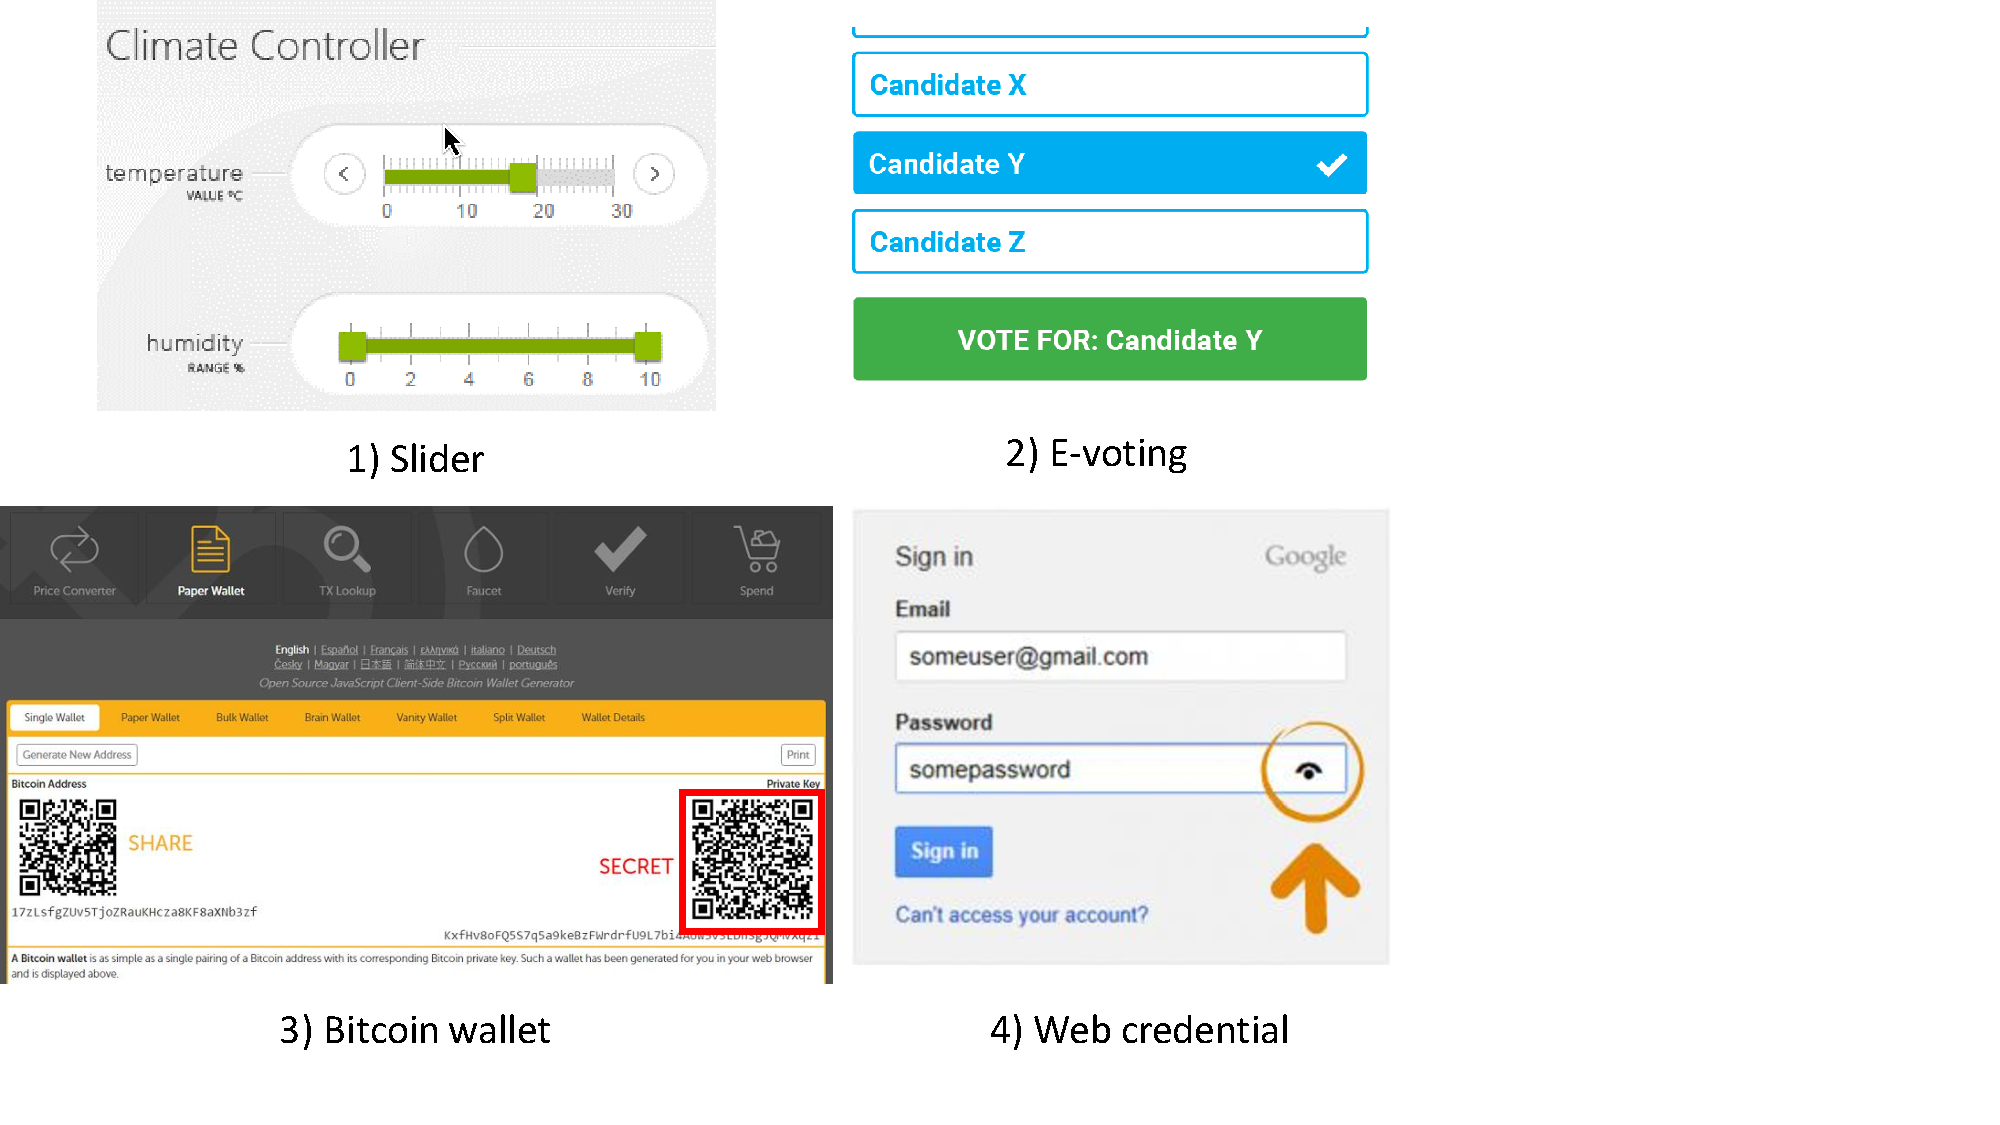
\includegraphics[trim={0 1cm 10cm 0}, clip, width=\linewidth]{motivation.pdf}
\caption{\textbf{Motivating examples.} 1) Pointer based UI elements that sets parameters to remote safety-critical device, 2) E-voting where the voting privacy and integrity is critical, 3) Financial transactions such as bitcoin wallet that shows sensitive information such as the user's private key and 4) web applications that provide an option for the user to reveal credentials.}
\spacesave
\label{fig:motivation}
\centering
\end{figure}
\fi

\begin{figure}[t]
\centering
%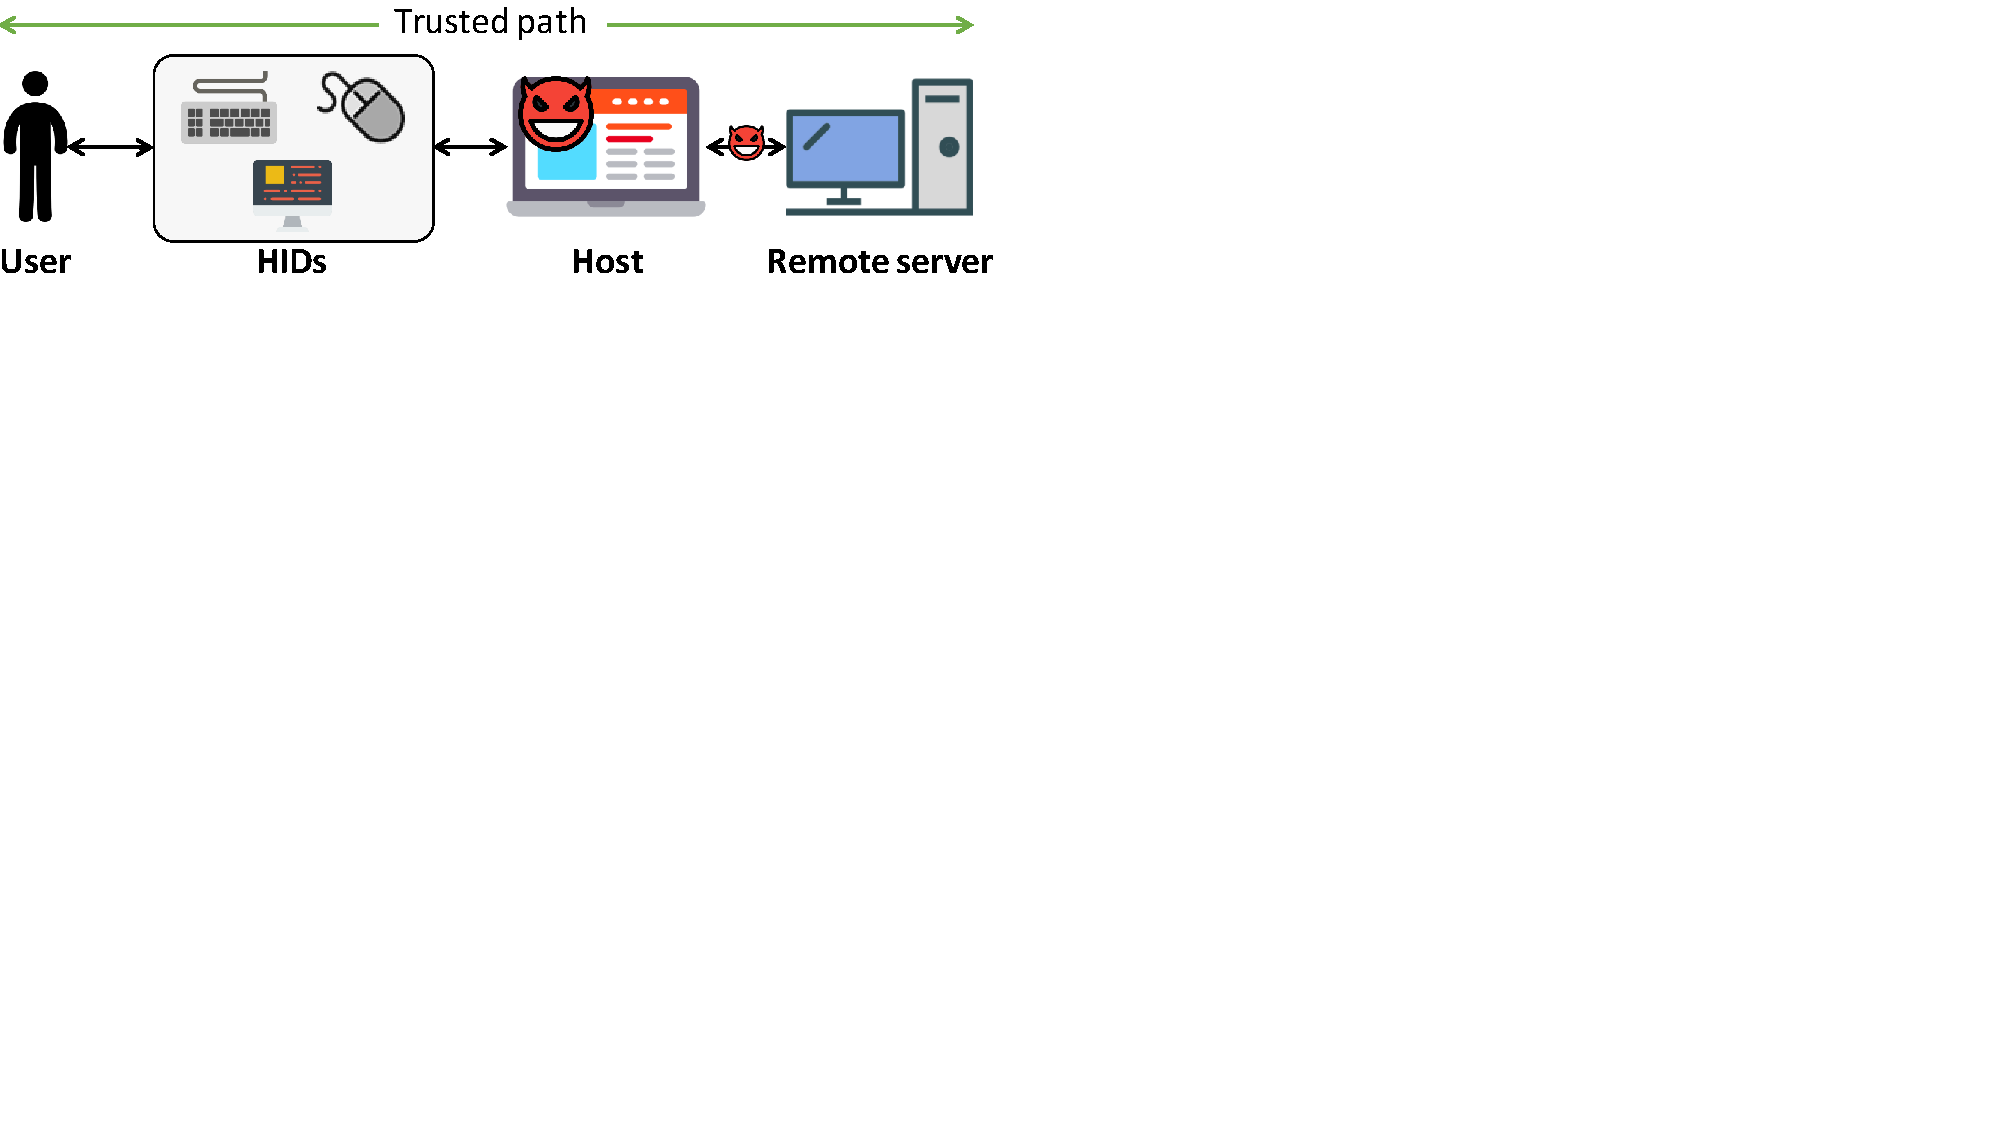
\includegraphics[trim={0 14cm 17cm 0}, clip, width=0.9\linewidth]{systemModel.pdf}
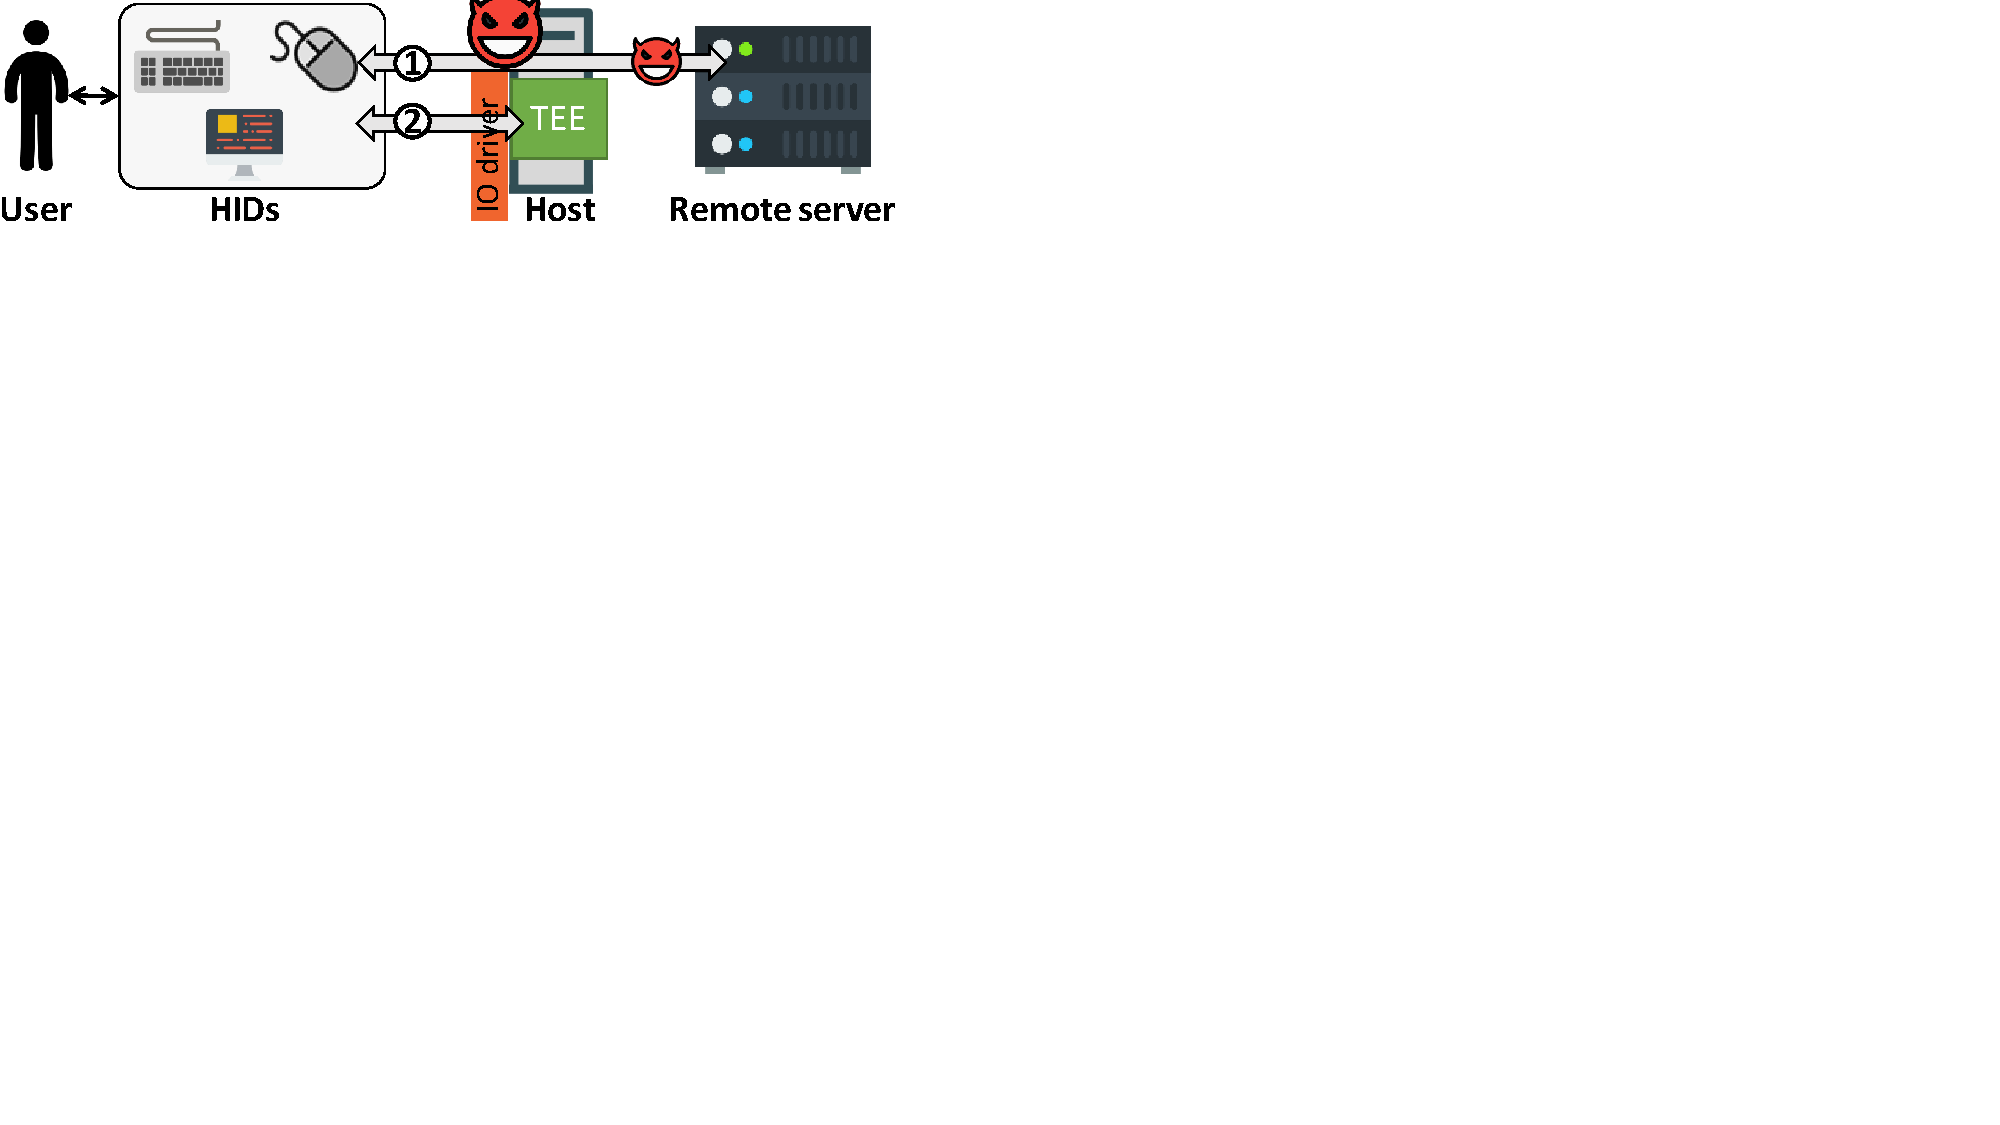
\includegraphics[trim={0 15cm 18cm 0}, clip, width=0.85\linewidth]{systemModel_all.pdf}
\caption{\textbf{Trusted path.} The figures shows the system and the attacker model of the trusted path. We generally consider two trusted path scenarios, \one trusted path to a remote server, and \two trusted path to a trusted execution environment (TEE) such as the Intel SGX.}
\spacesave
\label{fig:trustedPath}
\centering 
\end{figure}

%IO operation between the user and a remote server in the presence of an untrusted host is a long-standing problem. 
\emph{Trusted path} provides a secure channel between the user (specifically human interface device - HID) and the end-point, which is typically a trustworthy application running on the host. Trusted path ensures that user inputs reach the intended application unmodified, and all the outputs presented to the user are generated by the legitimate application. Trusted path to the local host is a well-researched area where many solutions focus on using trusted software components such as a trusted hypervisor. In work done by Zhou et al.~\cite{zhou2012building}, the authors proposed a generic trusted path on $x86$ systems with a pure hypervisor-based design. SGXIO~\cite{weiser2017sgxio} employed both the hypervisor and trusted execution environment (TEE) such as Intel SGX. However, hypervisors are hard to deploy, require a large TCB, and are impractical in real-world scenarios as most of the existing verified hypervisors offer a minimal set of features. 
%TEEs such as SGX rely on the OS to mediate IO operations and are also vulnerable to microarchitectural attacks~\cite{van2018foreshadow}.

Trusted external devices are another way to realize secure IO between a user and a remote server. Transaction confirmation devices~\cite{filyanov2011uni,weigold2011secure} allow the user to review her input data on a trusted device that is physically separated from the untrusted host. These approaches suffer from poor usability and are only limited to simple inputs. Bump in the Ether~\cite{McCPerRei2006} and IntegriKey~\cite{IntegriKey} use external embedded devices to sign input parameters. However, such solutions do not support output integrity; hence, the attacker can execute UI manipulation attacks to trick the user into providing incorrect inputs. Trusted overlay-based aproach~\cite{brandon2017trusted} uses a trusted FPGA to overlay UI elements such as a PIN entry screen on the LCD where the user can safely enter passwords.


Fidelius~\cite{Fidelius} combines the previous ideas of Bump in the Ether and trusted overlay to protect keyboard inputs from a compromised browser using external devices and a \js interpreter that runs inside an SGX enclave. Fidelius maintains overlays on display, specifically on the input text boxes to hide sensitive user inputs from the browser. We investigate the security of Fidelius and discover several issues. Fidelius imposes a high cognitive load to the users as they need to monitor continuously different security indicators (two LED lights and the status bar on the screen) to guarantee the integrity and confidentiality of the input. Furthermore, the attacker can manipulate labels of the UI elements to trick the user into providing incorrect input. Not supporting mouse also exposes Fidelius to early form submission attack where the host can emulate a mouse click on the submit button while the user is in the process of typing into the text field. This allows the attacker to perform an early form submission with incomplete input - a violation of input integrity. Fidelius is also vulnerable to microarchitectural attacks on SGX enclaves~\cite{van2018foreshadow} that extract attestation keys and relay attacks~\cite{dhar2018proximitee} that relay all user data to the attacker's platform. 

The drawbacks of the existing systems show that the problem of ensuring the integrity and confidentiality of the IO in the presence of an untrusted host is a non-trivial problem and requires a much more comprehensive solution. All of the previous trusted path solutions neither protect both input and output simultaneously, nor did they consider different modalities of input. We discuss such drawbacks in details, along with some of the relevant solutions in Section~\ref{sec:problemStatement:existingSolution}.

 
\myparagraph{Our contribution} The shortcomings of the existing literature provide the groundwork of our paper \name. %\name provides IO integrity and confidentiality guarantees without introducing major changes to the existing systems and user interaction and is generic across all the IO devices and a majority of the frequently used complex user interactions. 
\name is built on the idea that i) input integrity is is possible only when both input and output integrity are ensured simultaneously, ii) all the input modalities are needed to be protected as they influence each other, and iii) introducing low cognitive load on the users avoids user habituation errors. \name uses a trusted low-TCB auxiliary device that we call \device which works as a generic IO hub between all user IO devices and the untrusted host. \device does not to communicate with the trusted remote server. Instead, the \device uses the host as an untrusted transport.

\name ensures \emph{output integrity} and \emph{confidentiality} by sending an encoded UI to the host that only the \device can overlay on a small part of the screen. The overlay is possible as the \device intercepts the display signal between the host and the monitor. The overlay generated by the \device ensures that the host can neither observe nor manipulate any output information; hence, it can not trick the user. \device supports a subset of HTML5 UI elements that are frequently used in the majority of web applications. The \device also isolates the overlaid part of the screen by dimming out the rest when the user moves the mouse pointer on the overlaid UI. By doing so, \name aids the user to be more attentive to the security-critical UI on the screen. \name requires minor modification in the user interactions, and \name's active way to distinguish the trusted UI on the screen does not risk user habituation. 
%The \device analyzes the intercepted HDMI frames to understand the correct user context, such as if the user moves her mouse over a specific UI element and clicks there. %On top of the mouse pointer, the \device overlays another pointer that is visible to the user. In this way, \name mitigates clickjacking attacks~\footnote{In clickjacking attack the attacker spawns fake mouse pointer to trick the user into following it, while the legitimate mouse pointer is on a security-sensitive UI element}. The \device also intercepts the mouse and keyboard signals and match them with the display signal that is received from the untrusted host. If both the input and output co-relate, the \device signs all the input and sends them to the remote server. 
The input devices that are connected to the \device can only interact with the overlaid UI elements, making them completely isolated from the untrusted host. All the inputs are signed (and encrypt in case confidentiality is required) by the \device and sent to the remote server. \device is a fully plug-and-play device that is compatible with any host system regardless of their architecture or OS and does not require the user to install any software on the host. Note that our realization of \name uses an external device. However, the current system architecture can be modified, e.g., \device can be integrated into the graphics processor. We now summarize the contributions of \name as:


\begin{mybullet}
  \item The drawbacks in the literature provide the understanding that i) unless both output and input integrity are secured simultaneously, it is impossible to achieve any one of the two, and ii) without protecting the integrity of all the modalities of inputs, none could be achieved (refer to Section~\ref{sec:problemStatement:goals}). To our knowledge, \name is the first paper that provides such a concrete understanding. The paper also provides a formal security analysis in Appendix~\ref{appendix:security}. 
  \item We describe the design of \name, a system that provides a remote trusted path from the server to the user, in an attacker-controlled environment. The design of \name leverages a small, low-TCB auxiliary device that acts as a \emph{root-of-trust} for the IO. \name protects the integrity and confidentiality of the UI, specifically the integrity and confidentiality of mouse pointer and keyboard input. \name is further designed to avoid user habituation. Unlike transaction confirmation devices, \name can be used to protect complex IO interaction that are common in today's web forms with rich and complex UI elements e.g., radio-button, drop-down menu etc. (refer to Section~\ref{sec:systemDesign} \&~\ref{sec:confidentiality}).
  %\item We analyze the security of our solution in depth and argue why \name achieves IO integrity. We also discuss potential side-channel leakages that may undermine the confidentiality of IO (refer to Section~\ref{sec:securityAnalysis}). 
  \item We also implement a prototype of \name (that includes \device and \name \js) that is practical and easy to use (refer to Section~\ref{sec:prototype} \&~\ref{sec:eval}).
\end{mybullet}


\myparagraph{Organization of the paper} The organization of this paper is as the following. Section~\ref{sec:problemStatement} provides the detailed motivation, problem statement, state-of-the-art and the goals of this paper. Section~\ref{sec:approach} provides the system \& attacker model, challenges and a brief overview of our solution. We discussed the technical details of \name in Section~\ref{sec:systemDesign}. Section~\ref{sec:securityAnalysis} provides in-depth security analysis of \name. Section~\ref{sec:prototype} and~\ref{sec:eval} provide details of \name prototype implementation and corresponding evaluation. Finally, Section~\ref{sec:relatedWorks} and~\ref{sec:conclusion} provides the related research works and concludes the paper respectively.

 